% This must be in the first 5 lines to tell arXiv to use pdfLaTeX, which is strongly recommended.
\pdfoutput=1
% In particular, the hyperref package requires pdfLaTeX in order to break URLs across lines.

\documentclass[11pt]{article}
\usepackage{amsmath, adjustbox}
% Remove the "review" option to generate the final version.
\usepackage[review]{EMNLP2022}

% Standard package includes
\usepackage{times}
\usepackage{latexsym}

% For proper rendering and hyphenation of words containing Latin characters (including in bib files)
\usepackage[T1]{fontenc}
% For Vietnamese characters
% \usepackage[T5]{fontenc}
% See https://www.latex-project.org/help/documentation/encguide.pdf for other character sets

% This assumes your files are encoded as UTF8
\usepackage[utf8]{inputenc}

% This is not strictly necessary, and may be commented out.
% However, it will improve the layout of the manuscript,
% and will typically save some space.
\usepackage{microtype}

% This is also not strictly necessary, and may be commented out.
% However, it will improve the aesthetics of text in
% the typewriter font.
\usepackage{inconsolata}

\usepackage{graphicx}


% If the title and author information does not fit in the area allocated, uncomment the following
%
%\setlength\titlebox{<dim>}
%
% and set <dim> to something 5cm or larger.

\title{Using contradictions to improve QA systems}

% Author information can be set in various styles:
% For several authors from the same institution:
% \author{Author 1 \and ... \and Author n \\
%         Address line \\ ... \\ Address line}
% if the names do not fit well on one line use
%         Author 1 \\ {\bf Author 2} \\ ... \\ {\bf Author n} \\
% For authors from different institutions:
% \author{Author 1 \\ Address line \\  ... \\ Address line
%         \And  ... \And
%         Author n \\ Address line \\ ... \\ Address line}
% To start a seperate ``row'' of authors use \AND, as in
% \author{Author 1 \\ Address line \\  ... \\ Address line
%         \AND
%         Author 2 \\ Address line \\ ... \\ Address line \And
%         Author 3 \\ Address line \\ ... \\ Address line}

\author{First Author \\
  Affiliation / Address line 1 \\
  Affiliation / Address line 2 \\
  Affiliation / Address line 3 \\
  \texttt{email@domain} \\\And
  Second Author \\
  Affiliation / Address line 1 \\
  Affiliation / Address line 2 \\
  Affiliation / Address line 3 \\
  \texttt{email@domain} \\}

\begin{document}
\maketitle
\begin{abstract}
Ensuring the safety and interpretability of question answering (QA) systems is critical for deploying them in biomedical and scientific domains. One dominant approach to improving these systems uses natural language inference (NLI) to determine whether answers are entailed by some background context and thereby verifying the answer. Our work challenges this paradigm by looking at the dynamics of contradiction. We propose a contradiction-based system for answer ranking in multiple choice and extractive QA settings. Evaluating this system on a wide variety of datasets we find that while the contradiction-based system is competitive with and often better than entailment-only systems, a calibration model that incorporates contradiction, entailment, and QA model confidence scores outperforms other systems in all cases. Based on this result, we explore the unique opportunities for systems using contradiction on a wider scope of question answering such as improving interpretability and safety in open domain and generative settings.
\end{abstract}

\section{Introduction}
\begin{figure}
    \centering
  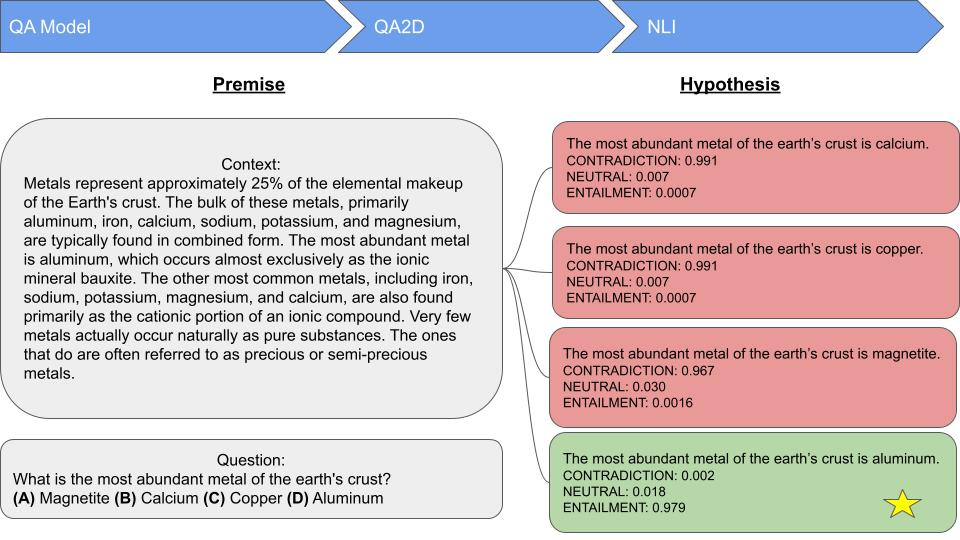
\includegraphics[width=1.0\linewidth]{EMNLP 2022/arch.jpg}
  \caption{A QA Model is used to produce answers for QA2D which reformulates answers as a hypothesis statement so that it can be used with an NLI model to determine whether the hypotheses are entailed or contradicted by the premise. Finally, the answers are ranked by the NLI class scores in various ways such as most entailed or least contradicted.}
  \label{fig:architecture}
\end{figure}
Safety in NLP systems is a major unresolved issue, particularly in biomedical and scientific contexts where known issues such as hallucination and overconfidence provide major obstacles to deploying them \citep{ji_survey_2022,kell_what_2021}. Utilizing natural language inference (NLI) as a method for improving the safety and performance of NLP research is an active area of research \citep{li_faithfulness_2022}. However, these systems typically focus exclusively on utilizing the entailment signal to verify answers. Similar research looks at building self-supporting NLP systems \citep{nakano_webgpt_2022, menick_teaching_2022} with the goal of improving safety by verifying model outputs with some external source.

We find these developments troubling since the critical rationalist philosophy of science \citep{miller_critical_2015} would predict that verification-based systems are not possible even in principle because statements can only be falsified with critical tests and never verified. Inspired by that prediction, we would like to explore refutation-based systems. In particular we look at an open research question: under NLI-based setups how do contradictions contribute to the performance and safety of question answering (QA) and how is this different from entailment or “verification” based systems. By exploring this question below, we hope to show why researchers should be critical of the paradigm of verification in NLP systems and why future work utilizing critical and contradicted statements could improve the safety of NLP systems.

We propose a method \ref{fig:architecture} that reformulates answers for multiple choice and extractive QA as hypothesis statements that can be criticized or critically tested against a premise given a NLI model. We then use the posterior probabilities of the QA and NLI models to rerank answers. We demonstrate that models fully calibrated with QA model confidence as well as entailment and contradiction scores outperform QA models by themselves in all cases. In addition, simply selecting the least contradicted answers with NLI only provides a competitive approach to selecting answers that is often on par with or better than entailment only systems. These results show that we should rethink the paradigm of verifying answers with entailment across NLP setups. While this work is in a relatively limited setting, we provide discussion on how leveraging contradictions could help improve open domain and abstractive QA as well as other NLP tasks at large.


\subsection{Related Work}

\textbf{NLI for QA} has been explored by several authors (see the overview in \citet{paramasivam_survey_2021}) showing performance improvements in multiple choice \citep{mishra_looking_2021}, extractive \citep{chen_can_2021}, open domain \citep{harabagiu_methods_2006} and multihop \citep{trivedi_repurposing_2019} settings. These approaches have thus far focused on using entailment as a verification mechanism. \citet{chen_can_2021} finds that under selective question answering \citep{kamath_selective_2020} for extractive QA, NLI systems can verify QA systems’ predictions. However, their result is limited to only selecting a top K \% of answers and doesn’t provide an approach for improving QA systems overall performance nor show what their results would have been like if they incorporated the contradiction signal. \citet{mishra_looking_2021} explores the use of entailment for multiple choice and fact checking settings and finds that not only do NLI models do well at these tasks by themselves but when they are adapted using in-domain data and longer premises they perform even better. Despite this, \citet{mishra_looking_2021} use a two class NLI set up (entailed v. not entailed) which means we don’t have any information about the effect of using the contradiction class.

\textbf{Factual consistency} is the only domain we are aware of that leverage contradictions directly from NLI. Factual consistency task seeks to ensure that a collection of utterances don't contain any contradictions such as hallucinations or unfaithfulness towards a source document (see \citet{li_faithfulness_2022} for an overview). Here approaches to improve factuality and faithfulness that use NLI are still mostly focused on entailment. \citet{laban_summac_2022} proposes a NLI-based method to ensure the consistency of a summary with a source document that incorporates contradiction and neutral scores with entailment scores beating out previous systems by a wide margin. Interestingly, they show that a combination of entailment and contradiction achieves the best results. Similarly, QAFactEval \citep{fabbri_qafacteval_2022} improves on \citet{laban_summac_2022} and maintains the approach of incorporating all NLI class scores not simply entailment. \citet{schuster_stretching_2022} and \citet{hsu_wikicontradiction_2021} develop interesting cases where contradictions are leveraged to identify contradictions within or across wikipedia articles illustrating the utility of contradictions. Finally, contradiction detection has surfaced as an important tool in generating dialogues that are consistent with a persona \citep{nie_i_2021, song_generating_2020}.

\textbf{Counterfactual, contrastive, and contradicted statements} are similar in that they provide statements which differ in some way from some original or expected statement. However, each is quite different in the context in which they are used. For counterfactual statements in a QA context, we ask what effect does a change in a context or question have on the answer, or what change in context or question is needed for a counterfactually perturbed answer \citep{kaushik_learning_2020}. Counterfactual statements are typically used to improve NLP systems by either augmenting datasets such that spurious correlations are avoided and better generalization is achieved or as a method for probing biases or performance gaps in already trained models \citep{gardner_evaluating_2020}. Contrastive statements on the other hand are designed to act as a negative sample in order to improve the representations learned during model training through contrastive learning \citep{schuster_get_2021, cao_cliff_2021}. Recently, works on fact verification have focused on generating statements that would be contradicted to build fact verification datasets \citep{wright_generating_2022, pan_contraqa_2021, saakyan_covid-fact_2021}. However these still act as negative samples during training. With contradicted statements, our primary concern is to have some statement that contradicts another statement without the need for it to be a perturbation of some original statement like a counterfactual or provide contrast to some positive sample for the purposes of training. Unlike works using counterfactual and contrastive statements, our concern with contradicted statements is primarily for improving systems at inference time which follows on the recent research program of deliberative reasoning \citep{bostrom_flexible_2021}.
\subsection{Contributions}
Our work provides the following contributions:
We propose a method that incorporates the contradiction signal in answer ranking for multiple choice and extractive QA setups
We show that across 9 multiple choice datasets and 7 datasets from MRQA 2019 \citep{fisch_mrqa_2019} a fully calibrated model that uses QA confidence scores as well as both entailment and contradiction score outperforms other setups and that a model calibrated with contradictions only is competitive with and even better than entailment only models in some settings.
We discuss how future work using contradicted statements can build systems with interpretability and inference procedures that are not possible with entailment based systems.

\section{Method}
\subsection{Overview}
We take a similar approach to \citet{chen_can_2021} and \citet{mishra_looking_2021} where we turn question answer pairs into declarative statements (QA2D) using a question answer to declarative statement model \citep{demszky_transforming_2018}. We then use a NLI model with a context passage as the premise and the declarative statement as a hypothesis. While the answers are provided for the multiple choice setting, we use an extractive QA model to produce answers for the extractive QA setting. We also use QA models for each setting to produce confidence scores which are later used to train calibration models.

Once we have a three class NLI classification (entailment, neutral, contradiction), we use the confidence for the classification as a signal for ranking answers. Like \citet{chen_can_2021} we use a calibration method that combines the confidence scores from the QA models and the NLI classification confidence scores using logistic regression trained on a hold out set. In the multiple choice setting, we rank answers for answer selection. In the extractive QA case, we rank questions for selective QA \citep{kamath_selective_2020} where we select a top K number of answers by how confident the model is in answering that question.
\subsection{QA Models}
For the multiple choice setting, we wanted to test how the proposed architecture performs under domain shifts so we used RoBERTa large \citep{liu_roberta_2019} fine tuned on the race dataset as well as two DeBERTa v3 \citep{he_debertav3_2021} variants (base and xsmall) on SciQ. For the extractive QA setting, we used DistillBERT \citep{sanh_distilbert_2020} and BERT-Large \citep{devlin_bert_2019}) models trained on SQuAD \citep{rajpurkar_squad_2016}. More details on training and validation are available in Appendix A.
\subsection{QA2D}
A QA2D model reformulates a question-answer pair to a declarative statement \citep{demszky_transforming_2018}. As noted in \citet{chen_can_2021} and \citet{mishra_looking_2021}, the QA2D reformulation is critical to using NLI models in a QA since we need to have the proposed answer match the format of NLI which requires declarative statements as hypothesis. More formally, we would like to transform a question answer pair $(q, a)$ to a truth conditional hypothesis H such that H is found to be entailed (P⊢H), contradicted (P⊥H), or neither entailed nor contradicted (P or H) by some premise P. 

We trained a T5-small model \citep{raffel_exploring_2020} on the dataset proposed by \citet{demszky_transforming_2018} for QA2D since we found almost no noticeable differences in performance in larger models. Unlike \citet{chen_can_2021}, we found that regardless of size, these QA2D models struggled with long questions or questions with complex syntax and would often leave the answer out of the statement. The same result occurred when we directly used the model trained by \citet{chen_can_2021}. In order to solve this, we tried using constrained decoding that required the answer to be in the statement. However, this often produced ungrammatical or nonsensical statements. We settled with the following heuristic to postprocess QA2D outputs: If less than 50\% of the tokens in the answer were in the statement then we appended the answer to the end of the statement. We used 50\% to account for rephrasing the answer or swapping pronouns. While some statements resulted in answer redundancy, we felt that this was better than having hypotheses which left out the answer statement. Future work on QA2D should focus on how we can use these models outside of the domains in the dataset provided by \citet{demszky_transforming_2018}.
\subsection{NLI}
Since we’d like to know whether the reformulated answer statement is contradicted, entailed, or neutral w.r.t to the context passage, we used a series of NLI models to test each context passage against the reformulated answer statements. We used the whole context as \citet{schuster_stretching_2022} and \citet{mishra_looking_2021} demonstrated that long premises still performed adequate though not as well as sentence-length premises.
We used two DeBERTa-based models \citep{he_deberta_2021} trained on the MNLI dataset (called mnli-base and mnli-large) and an albert model trained on the ANLI dataset in addition to various other NLI datasets (called albert-anli) \citep{nie_adversarial_2020}. Using these models we performed NLI on the context passages as the premise and the reformulated answer statement as the hypothesis for each answer in both the multiple choice and extractive QA settings. The confidence scores for each class are then used for downstream ranking.
\subsection{Calibration Models}
Like \citet{kamath_selective_2020} and \citet{chen_can_2021} we developed a set of calibration models in order to do answer ranking. A calibration model is trained on a set of posterior probabilities from downstream models to predict whether an answer is correct. The calibration model can then combine a set of downstream models for its ultimate prediction. Since we want to compare the effect of using NLI class confidence scores we trained the following set of models. QA indicates that the QA model confidence score is being used, E indicates the entailment score is used, C indicates the contradiction score is used and N indicates the neutral score. QA + X, indicates a linear combination of QA confidence scores and a set of NLI class confidences. Finally we also try calibration with entailment and contradiction E + C. Like \citet{chen_can_2021} all calibration models are trained on a holdout set of 100 samples from a single domain using logistic regression where we predict whether, given the confidence scores of the downstream models, the answer is correct. To illustrate what is learned Appendix D presents a regression analysis for the multiple choice setting.
\subsection{Answer Ranking}
Similar to \citet{harabagiu_methods_2006}, we rank the answers based on the highest probability from the calibration model $\sigma$ given a linear combination of the QA or NLI scores given an answer $n \in N$. Where we only select a single NLI class or QA class no calibration is used and $\sigma$ is simply the identity of the confidence score. In the case of contradiction only $\sigma$ is the inverse of the contradiction confidence score, indicating we are selecting the least contradicted answer. 

$$
\underset{N}{\operatorname{argmax}}\:\sigma(QA_n;NLI_n)
$$
For the multiple choice setting we used this for selecting the answer to a given question. We found that using a top $K=4$ approach to extractive QA generated almost the same answers with slightly different spans so we did not use the approach with extractive QA. For both the multiple choice and extractive QA settings we ranked answers by each model as answering the question as in \citet{kamath_selective_2020}. We used this ranking to select a top $n$ set of questions, called coverage, to answer so we could compare each approach at various coverage thresholds.
\subsection{Datasets}
For both settings, we used datasets where the context passage the answer is found in is already available. We also wanted to be sure we selected a wide variety of datasets for each setting so we could test the viability of our approach and provide results that could be compared with \citet{chen_can_2021} and \citet{mishra_looking_2021}. The multiple choice setting we used a comprehensive set of 9 datasets. Two of those datasets are in-domain for the QA and calibration, RACE and SciQ. For the extractive QA case we used 5 of the datasets from the MRQA 2019 task \citep{fisch_mrqa_2019} as well as SQuAD2.0 \citep{rajpurkar_know_2018} and SQuAD adversarial \citep{jia_adversarial_2017} for a total of 7 extractive QA datasets. The in-domain dataset for the extractive QA model is SQuAD and the dataset used for calibration is Natural Questions since that is what was used by \citet{chen_can_2021}. The only preprocessing done was to remove questions where the context was empty. Appendix B describes full details on the datasets used for evaluation.
\section{Results}
\subsection{Ranking multiple choice}
\begin{table*}[]
\centering
\begin{tabular}{lllllllllll}
\hline
Model & Cosmos & Dream & MCS & MCS2 & MCT & QASC & RACE & R_C & SciQ & Avg \\ \hline
S-base & 18.46 & 43.80 & 61.99 & 63.71 & 44.76 & 93.41 & 30.97 & 27.39 & 95.28 & 53.30 \\
S-small & 25.46 & 48.26 & 60.28 & 66.04 & 59.76 & 90.60 & 35.56 & 30.62 & 98.09 & 57.18 \\
RACE & 64.22 & 82.56 & 89.70 & 86.98 & 90.48 & 98.16 & 76.93 & 69.80 & 97.96 & 84.08 \\
E+C & 44.36 & 80.94 & 85.52 & 84.99 & 90.60 & 96.44 & 64.29 & 51.40 & 92.47 & 76.77 \\
E & 36.18 & 79.03 & 86.02 & 79.72 & 89.88 & 95.90 & 62.14 & 49.72 & 91.96 & 74.50 \\
C & 59.26 & 78.98 & 83.12 & 84.43 & 89.29 & 92.76 & 62.74 & 47.05 & 91.58 & 76.58 \\ \hline
\end{tabular}
\caption{Accuracy scores on NLI-only answer ranking. The best scores are bold and the second best are underlined.}
\label{tab:nli_only_performance}
\end{table*}

\begin{table*}[]
\centering
\begin{tabular}{lllllllllll}
\hline
model & Cosmos & Dream & MCS & MCS2 & MCT & QASC & RACE & R_C & SciQ & Avg \\ \hline
s-base & 18.46 & 43.80 & 61.99 & 63.71 & 44.76 & 93.41 & 30.97 & 27.39 & 95.28 & 53.30 \\
s-small & 25.46 & 48.26 & 60.28 & 66.04 & 59.76 & 90.60 & 35.56 & 30.62 & 98.09 & 57.18  \\
RACE & 64.22 & 82.56 & 89.70 & 86.98 & 90.48 & 98.16 & 76.93 & 69.80 & 97.96 & 84.08 \\
QA+E+C & 64.72 & 83.19 & 90.06 & 87.59 & 91.43 & 98.60 & 77.53 & 69.80 & 98.21 & 84.57 \\
QA+E & 64.32 & 82.85 & 89.92 & 87.29 & 91.07 & 98.49 & 77.18 & 69.66 & 98.09 & 84.31 \\
QA+C & 64.82 & 82.75 & 89.88 & 87.29 & 90.83 & 98.38 & 77.16 & 69.80 & 98.09 & 84.33 \\ \hline
\end{tabular}
\caption{Accuracy scores on calibrated NLI answer ranking. Calibrations are with the RoBERTa-RACE model. The best scores are bold and the second best are underlined.}
\label{tab:calibrated_performance}
\end{table*}
In tables \ref{tab:nli_only_performance} (NLI only) and \ref{tab:calibrated_performance} (calibrated) we present the accuracy achieved on each of the 9 datasets. We show results with each QA model and the mnli-large model for NLI (Appendix C shows results for alberta-anli and mnli-base which perform worse but generally reflect the same trends). On the NLI-only results presented in table \ref{tab:nli_only_performance}, the QA model only on race outperforms on most datasets except MCTest and the combination of entailment and contradiction tends to do second best. Notably, the SciQ models do much worse than the NLI only ranking for either class except on in-domain questions for SciQ and the similar QASC dataset. We think this indicates that the race domain is more generic than the SciQ domain. These results show that an NLI-only approach can be competitive with a robust QA model and better than a QA model trained in a specific domain. Notably, we also show that incorporating the contradiction scores with the entailment scores is better than entailment alone and that selecting the least contradicted answer is quite competitive with selecting the most entailed answer. Additionally, other than the RACE QA model, the contradiction model has the lowest variance of 2.65\% indicating that selecting the least contradicted answer may help with more stable performance across domains.
When we look at the results from the calibration models we see that the NLI calibrated models outperform the QA only in all cases (in-domain with race where they perform the same). The best calibration incorporates the QA confidence, entailment, and contradiction (QA + E + C) achieving an average accuracy of 84.57\% over 84.09\% achieved by the RoBERTa-RACE. The second best approach is the calibration with contradiction only (84.33\%), however only slightly over entailment only (84.32\%). Although only slightly less than the QA model (1.4\%) the calibration with contradiction only achieves the lowest variance of 1.3\% lending support to the finding above that selecting the least contradicted answer may help with generalization.
\subsection{Selective QA}
\begin{table*}[]
\centering
\begin{tabular}{lllllllll}
\hline
 & Database & QA + E + C & QA + C & QA + E & E + C & E & C & QA \\ \hline
20\% & CosmosQA & 77.55 & 91.12 & 76.88 & 69.18 & 68.34 & 83.25 & 88.61 \\
 & DREAM & 98.28 & 98.77 & 98.28 & 96.32 & 96.32 & 96.81 & 98.28 \\
 & MCScript & 99.82 & 99.46 & 99.82 & 99.64 & 99.64 & 99.46 & 99.82 \\
 & MCScript-2.0 & 99.58 & 99.72 & 99.45 & 99.17 & 99.03 & 97.37 & 99.58 \\
 & MCTest & 100 & 99.40 & 100 & 100 & 100 & 99.40 & 98.81 \\
 & QASC & 100 & 100 & 100 & 100 & 100 & 100 & 100 \\
 & RACE & 94.93 & 96.69 & 94.72 & 92.44 & 92.24 & 90.17 & 98.24 \\
 & R_C & 88.73 & 92.96 & 89.44 & 85.21 & 85.92 & 86.62 & 93.66 \\
 & SciQ & 100 & 100 & 100 & 100 & 100 & 100 & 100 \\
 & avg & 95.43 & 97.57 & 95.40 & 93.55 & 93.50 & 94.79 & 97.45 \\
50\% & CosmosQA & 80.29 & 81.70 & 76.94 & 75.80 & 70.64 & 80.63 & 76.47 \\
 & DREAM & 95.10 & 96.86 & 94.90 & 93.63 & 93.63 & 93.63 & 96.67 \\
 & MCScript & 98.57 & 98.64 & 98.28 & 98.00 & 97.93 & 97.14 & 98.78 \\
 & MCScript-2.0 & 96.40 & 98.23 & 95.84 & 94.68 & 94.40 & 96.01 & 98.01 \\
 & MCTest & 99.52 & 99.76 & 99.52 & 99.05 & 99.05 & 99.76 & 99.52 \\
 & QASC & 100 & 100 & 100 & 99.78 & 99.78 & 99.78 & 100 \\
 & RACE & 90.11 & 92.68 & 89.99 & 87.71 & 87.38 & 85.23 & 93.88 \\
 & R_C & 85.11 & 84.83 & 85.39 & 78.37 & 78.37 & 77.25 & 87.36 \\
 & SciQ & 100 & 100 & 100 & 100 & 100 & 99.74 & 100 \\
 & avg & 93.90 & 94.74 & 93.43 & 91.89 & 91.24 & 92.13 & 94.52 \\ \hline
\end{tabular}
\caption{Selective QA for the multiple choice with accuracy scores at 20\% and 50\%. Calibrations and QA confidence are all from RoBERTa-RACE where RACE is the in-domain dataset.}
\label{tab:selective_mc_qa}
\end{table*}
For selective QA evaluation in both settings, the QA model selects the answer and then we evaluate the top 20\% or 50\% of those answers after sorting them by the approaches we outlined above. In the multiple choice setting we do not select the answers with the ranking as proposed in the method above since the results were not underperformed. Those results are available in Appendix C.
\subsubsection{Selective QA in the Multiple Choice Setting}
In table \ref{tab:selective_mc_qa}, the first thing to note is that the QA + C model performs the best on selective QA, achieving best or second best accuracy on almost every dataset for an average of 97.57\% at 20\% coverage and 94.74\% at 50\% coverage over 97.45\% at 20\% coverage and 94.52\% at 50\% coverage achieved by the RoBERTA-RACE QA model. This is especially striking at 50\% coverage where the QA model only does significantly better on the in-domain race datasets. The contradiction calibration model is also the only model to outperform the QA model ranking by confidence score. While the NLI only models can be competitive with the calibrated models, we also highlight that sorting by the least contradicted achieves quite good performance and is often quite a bit better (94.79\% @ 20\% / 92.13\% @ 50\%), than sorting by the most entailed (93.50\% @ 20\% / 91.24\% @ 50\%) or a combination of entailed and contradicted (93.55\% @ 20\% / 91.89\% @ 50\%). These results would be inline with our intuition that the less contradicted an answer is the more likely it is correct even in cases where we might be uncertain about its entailment.
\subsubsection{SelectiveQA in the extractive QA settings}
\begin{table*}[]
\centering
\begin{tabular}{lllllllll}
\hline
 & Dataset & QA + E + C & QA + E & QA + C & E + C & E & C & QA \\ \hline
20\% & BioASQ & 85.04 & 85.06 & 83.10 & 74.22 & 74.22 & 75.47 & 82.99 \\
 & HotpotQA & 86.62 & 86.69 & 85.89 & 80.60 & 80.60 & 79.82 & 85.33 \\
 & NaturalQuestions & 91.84 & 91.68 & 92.18 & 79.89 & 79.87 & 82.09 & 90.98 \\
 & SQuAD & 98.26 & 98.76 & 98.17 & 92.37 & 92.48 & 90.88 & 99.04 \\
 & squad\_adversarial & 43.99 & 43.98 & 43.57 & 43.74 & 43.60 & 42.81 & 39.83 \\
 & squadv2 & 37.64 & 37.56 & 36.07 & 37.43 & 37.31 & 37.68 & 30.52 \\
 & TriviaQA & 81.33 & 81.21 & 80.36 & 65.53 & 65.25 & 69.13 & 80.68 \\
 & avg & 74.96 & 74.99 & 74.19 & 67.68 & 67.62 & 68.27 & 72.77 \\
50\% & BioASQ & 76.13 & 76.04 & 75.51 & 71.49 & 71.49 & 72.97 & 75.49 \\
 & HotpotQA & 79.37 & 79.30 & 78.95 & 77.43 & 77.43 & 77.31 & 78.74 \\
 & NaturalQuestions & 84.53 & 84.48 & 83.24 & 74.96 & 74.93 & 78.62 & 82.47 \\
 & SQuAD & 96.98 & 96.97 & 97.01 & 91.58 & 91.52 & 91.19 & 97.00 \\
 & squad\_adversarial & 41.80 & 41.16 & 41.49 & 42.76 & 42.79 & 42.03 & 40.26 \\
 & squadv2 & 29.41 & 28.45 & 28.77 & 34.43 & 34.14 & 34.39 & 26.18 \\
 & TriviaQA & 74.30 & 74.37 & 74.23 & 65.05 & 64.93 & 68.08 & 74.21 \\
 & avg & 68.93 & 68.68 & 68.46 & 65.39 & 65.32 & 66.37 & 67.76 \\ \hline
\end{tabular}
\caption{Selective QA for extractive QA with F1 scores at 20\% and 50\% coverage. Calibrated models and QA use the BERT-large model.}
\label{tab:selective_extractive_qa}
\end{table*}
For the extractive QA setting we present the same analysis in table \ref{selective_extractive_qa}. We do observe similar trends as above where calibration with contradiction only, QA + C, has quite a bit better average F1 scores than the QA model (74.19\% vs 72.77\% at 20\%, 68.46\% vs 67.76\% at 50\%). Of the NLI-only ranking, selecting the least contradicted does best. Although only slightly better than the QA + C, the results show that the QA + E model does best at 20\% coverage and the QA + E + C model does best at 50\% coverage. This indicates that entailment is still an important signal, albeit more powerful when combined with contradiction. Appendix C contains a comparison with the smaller DistillBERT model which shows similar results.
\subsection{Answer Rejection on SQuAD 2.0}
\begin{table*}[t!]
\centering
\begin{tabular}{llllll}
\hline
 & rejects & accepts & precision & recall & f1 \\ \hline
QA \textless 50\% & 46.71\% & 86.15\% & 62.81\% & 23.39\% & 34.09\% \\
QA \textless 25\% & 22.29\% & 95.45\% & 71.05\% & 11.16\% & 19.29\% \\
QA  \textless 75\% & 71.22\% & 72.86\% & 56.79\% & 35.66\% & 43.81\% \\
E \textless 5\% & 43.80\% & 98.74\% & 94.55\% & 21.93\% & 35.61\% \\
E \textless 25\% & 63.82\% & 96.58\% & 90.33\% & 31.95\% & 47.21\% \\
E \textless 10\% & 52.14\% & 98.02\% & 92.95\% & 26.11\% & 40.77\% \\
E \textless  50\% & 76.94\% & 91.52\% & 81.96\% & 38.52\% & 52.41\% \\
C \textgreater 50\% & 42.78\% & 99.35\% & 97.06\% & 21.42\% & 35.09\% \\
C \textgreater 25\% & 54.21\% & 98.59\% & 95.05\% & 27.15\% & 42.23\% \\
C \textgreater 10\% & 66.88\% & 96.50\% & 90.53\% & 33.49\% & 48.89\% \\
C \textgreater  5\% & 76.15\% & 93.23\% & 84.92\% & 38.13\% & 52.63\% \\ \hline
\end{tabular}
\caption{Rejecting unanswerable questions in SQuAD2.0 (11,873 answers total with 5,945 unanswerable questions). Bold indicates the best score and underlined indicates the second best score.}
\label{tab:rejecting}
\end{table*}
In order to explore how useful contradiction might be over other setups, we evaluated the answer rejection task in SQuAD 2.0 \citep{rajpurkar_know_2018} using our BERT-large model. This task evaluates how well a model does at abstaining from answering a question when there is no gold answer. We selected three setups, rejecting answers by QA confidence, by entailment score, and by contradiction score. Notably, when we select by least entailed answers we end up treating the problem as two class NLI (entailed v not entailed) which was previously looked at by \citet{chen_can_2021}.
Table \ref{tab:rejecting} shows that the NLI-based setups outperform QA confidence setups in all cases. Interestingly, the difference between rejecting answers that are not entailed and rejecting answers that have been contradicted appears to reflect a precision versus recall tradeoff. The overall model (best F1 score) is achieved by rejecting answers where the contradiction score was greater than 5\% successfully rejecting 76.15\% answers and accepting 93.23\% answerable questions. Rejecting answers if they are not entailed, where E < 50\%, achieves the second best F1 score and illustrates an interesting dynamic. E < 50\% has the best recall (38.52\%), successfully rejects the most answers, while C > 50\% has the best precision (97.06\%), accepting the most answerable questions. This result shows that if we want to build systems that err on the side of rejecting correct answers then selecting answers that are not entailed has an advantage. Conversely, if we want to build systems that are better at rejecting only answers that should be rejected then rejecting contradicted answers is a better strategy. Interestingly our results highlight the utility of using contradiction confidence scores even if they are low which gives credence to using the contradiction score as a meaningful signal.
\subsection{Correlation Analysis}
\begin{table*}[]
\centering
\begin{tabular}{llllllll}
\hline
 &  & Contradiction &  & Entailment &  & Neutral &  \\ \hline
Dataset & QA & score & class & score & class & score & class \\
CosmosQA & 0.53 & -0.34 & -0.17 & 0.05 & -0.01 & 0.21 & 0.16 \\
DREAM & 0.72 & -0.57 & -0.35 & 0.54 & 0.50 & -0.11 & -0.13 \\
MCScript & 0.80 & -0.59 & -0.42 & 0.59 & 0.50 & -0.04 & -0.08 \\
MCScript2 & 0.77 & -0.50 & -0.32 & 0.41 & 0.37 & -0.04 & -0.05 \\
MCTest & 0.73 & -0.65 & -0.47 & 0.64 & 0.69 & -0.20 & -0.15 \\
QASC & 0.57 & -0.54 & -0.28 & 0.55 & 0.67 & -0.50 & -0.26 \\
RACE & 0.65 & -0.37 & -0.20 & 0.35 & 0.34 & -0.11 & -0.11 \\
RACE-C & 0.59 & -0.24 & -0.13 & 0.18 & 0.25 & -0.09 & -0.11 \\
SciQ & 0.75 & -0.69 & -0.47 & 0.68 & 0.67 & -0.42 & -0.19 \\ \hline
\end{tabular}
\caption{Correlation analysis (spearman rank correlation) per dataset in the multiple choice setting. RoBERTa-RACE is used for the QA scores.}
\label{tab:per_dataset_correlation}
\end{table*}
\begin{table*}[]
\centering
\begin{tabular}{llllll}
\hline
 &  & contradiction & entailment & neutral & QA \\ \hline
multiple choice & Confidence & -0.47 & 0.37 & -0.06 & 0.71 \\
 & Class & -0.28 & 0.38 & -0.06 &  \\
extractive QA & Confidence & -0.16 & 0.31 & -0.12 & 0.19 \\
 & Class & -0.15 & 0.39 & -0.29 &  \\ \hline
\end{tabular}
\caption{Correlation analysis (spearman rank correlation) in the multiple choice and extractive QA settings. RoBERTa-RACE is the QA model used for multiple choice QA scores and BERT-large is used for the extractive QA scores.}
\label{tab:correlation}
\end{table*}
Since we are using the NLI and QA model scores to construct the setups above, we’d like to know how these factors correlate with the correct answer. Table \ref{tab:correlation} shows how each NLI class correlates both by score and by actual classification (score > 50\%) as compared against QA model confidence score. The multiple choice analysis shows answers from the RoBERTa-RACE model and the extractive QA analysis shows answers from the BERT-large model trained on SQuAD. The correlation analysis presents spearman rank correlations. What we see below is that in the multiple choice setting the confidence score has a strong correlation with the correct answer which makes sense given the confidence score is a softmax over the multiple choice classes. Extractive QA confidence scores have a much weaker correlation and tend to have less correlation than entailment has with the correct answer. Despite the results presented above, contradiction only has a notable correlation with the correct answer when the confidence score is used in the multiple choice setting justifying our answer ranking approach. Interestingly in the extractive QA case the neutral class is more negatively correlated when selecting by classification. Our conjecture would be that in the extractive QA case we don’t have much to compare against. When looking at the per dataset correlations for the multiple choice setting (Table \ref{tab:per_dataset_correlation}) we see that in most cases, other than the QA confidence scores, the contradiction scores have the strongest correlations with the correct answer out of any NLI class and neutral, as we would expect, tends to have very weak correlations.
\section{Discussion}
\subsection{Contradiction as a Signal}
Contradiction is a particularly important signal because it lends interpretability to systems taking advantage of it. If we are choosing answers based on the least contradicted answer, we have information about the other answers and why we didn’t select them. Namely, that they were contradicted. Entailment and QA model confidence do not have the same interpretability since all we know about the other answers is they have a lower entailment or confidence score, they could still be correct or entailed. In addition, we would not know if they were neutral or contradicted with respect to the premise.
Once we know an answer is contradicted we can also use that information to try retrieving another answer or we can use that answer to modify a prompt to indicate the model should use it as a hint that the answer is not the correct one. Entailment does not lend itself to this iterative refinement of question answering and we suggest that future work on utilizing contradiction should investigate developing inference techniques that take advantage of the contradiction signal.
Contradiction also provides a unique opportunity for open domain QA systems where we need to retrieve a context containing the answer. Like entailment-based approaches (Harabagiu and Hickl, 2006) we can try selecting the least contradicted passage for a downstream reader. We can also imagine extending the work of \citet{schuster_stretching_2022} where contradiction-based approaches could be used to retrieve passages that would contradict an answer to determine if the proposed answer might be wrong and thereby develop an iterative inference procedure for open domain settings.
Finally contradicted statements are already being used in a generative setting to improve fact verification systems during train time \citep{wright_generating_2022, pan_zero-shot_2021, saakyan_covid-fact_2021}. Recent work \citep{saunders_self-critiquing_2022} has shown that self-criticism is a powerful technique for improving the quality of NLP systems during inference and we believe generating critical statements for model predictions could help with overall performance, interpretability, and safety. Future work should assess whether a refutation-based paradigm to improve NLP safety along these lines is an interesting alternative to the current verification-based one.
\section{Limitations}
Despite the results above, multiple choice QA and extractive QA with a provided context is a limited setting that doesn’t indicate the results would extend to other popular settings where NLI are used such as abstractive QA, summarization, factual consistency and so on. We are hopeful given that \citet{laban_summac_2022} shows similar results that contradiction is an important signal in factual consistency. The primary problems that we envision with the approach as we have outlined it are presented below.
\subsection{Context Length and NLI Datasets}
Even though there is a greater tendency to use NLI in zero-shot settings \citep{yin_universal_2020}. Domain transfer is a known issue with using NLI models. In particular, NLI datasets tend to focus on textual entailment over short passages such as sentence pairs and performance degrades when using longer passages such as in the datasets we use \citep{mishra_looking_2021}. Even when in-domain datasets are created \citep{chen_can_2021, khot_scitail_2018, mishra_looking_2021}. They tend to focus on data augmentation strategies that produce two-class NLI datasets (entail, not entailed) which wouldn’t give us any contradiction signals. Future work should pick up on producing models capable of performing textual entailment over longer passages and devising methods for generating three-class NLI datasets so that we can determine if contradictions receive the same benefits from those approaches that entailment has. Additionally we saw that albert-anli performed worse than mnli-large and mnli-large performs poorly on some datasets indicating that we still have much more work to do to improve upon NLI in general.
\subsection{Ranking requires alternatives and time}
In the extractive QA setting presented above we cannot use ranking to select an answer we introduced for the multiple choice setting without developing QA models that have more diverse outputs. Like other textual entailment based systems, this speaks to the computational expense involved in generating and evaluating answer alternatives. If we were to apply our method to an open domain setting where a set of context passages are retrieved, the ranking procedure would require a quadratic evaluation procedure for each context passage against each reformulated answer candidate \citep{schuster_stretching_2022}. Future work should look towards comparison approaches that amortize the computational cost involved in pairwise NLI based ranking techniques such as investigating NLI-based dense passage retrieval \citep{reimers_sentence-bert_2019}.
\section{Summary}
We have demonstrated that incorporating contradiction is an important signal for multiple choice and extractive QA systems. By proposing a method that reformulates answers as hypothesis statements, we were able to rank answers and demonstrate that QA model confidence calibrated with entailment and contradiction scores outperform QA models by themselves in all cases. In addition, models calibrated with contradiction only or simply selecting the least contradicted answers with NLI only provides a competitive approach to selecting answers that is often on par with or better than entailment only systems. These results show that we should rethink the paradigm of verifying answers with entailment across NLP setups. While this work is in a relatively limited setting, we provide discussion on how leveraging contradictions could help improve open domain and abstractive QA as well as other NLP tasks at large.

\section{Ethics Statement}
Works addressing NLP safety should be aware of their limitations and be clear about potential harms and misuse of their proposed approaches. Systems that improve safety by verification or support are vulnerable to drawing on untrue and biased sources to justify their outputs. The appearance of credibility given to texts that use citations and appeals to authority means that we should make users aware that the sources they draw on can be wrong. This applies to critical sources as well since a source can provide criticism that is wrong. However, by presenting contradictions we do believe that systems of this nature could provide a wider breadth of criticism and engage users critical reasoning more readily than models which claim to verify answers by appealing to the authority of some source document.

% Entries for the entire Anthology, followed by custom entries
\bibliography{anthology,custom}
\bibliographystyle{acl_natbib}

\appendix

\section{Training Setup and Reproducibility}
\label{sec:appendix}

\begin{table*}[]
\centering
\begin{tabular}{lll}
\hline
Huggingface name & Name \\ \hline
LIAMF-USP/roberta-large-finetuned-RACE & RoBERTa-RACE \\
bert-large-uncased-whole-word-masking-finetuned-squad & BERT-Large \\
distilbert-base-uncased-distilled-squad & DistillBERT \\
ynie/albert-xxlarge-v2-snli\_mnli\_fever\_anli\_R1\_R2\_R3-nli & albert-anli \\
microsoft/deberta-base-mnli & mnli-base \\
microsoft/deberta-v2-xxlarge-mnli & mnli-large \\ \hline
\end{tabular}
\caption{Pretrained models that we used.}
\label{tab:models_trained}
\end{table*}

\begin{table*}[t]
\centering
\begin{tabular}{lllll}
\hline
Model & Dataset & Epochs & Score &  \\ \hline
t5-small & Demszky et al. (2018) & 20 & Rogue1 & 90.73 \\
deberta-v3-xsmall & Welbl et al. (2017) & 6 & Accuracy & 93.99 \\
deberta-v3-base & Welbl et al. (2017) & 6 & Accuracy & 91.79 \\ \hline
\end{tabular}
\caption{The models we trained for or setups with evaluation scores and number of epochs trained.}
\label{tab:models_trained}
\end{table*}
Table \ref{tab:models_trained} outlines the pretrained models that we used and datasets they are trained on, all of these models are publicly available on the huggingface model hub.
In addition to several pretrained models used in the setups described earlier, we trained 3 models, a t5-small model on \citet{demszky_transforming_2018} for the QA2D set up where a Rogue1 of 90.73\% is achieved on the validation set, deberta-v3 models (xsmall and base) trained on SciQ \citep{welbl_crowdsourcing_2017} achieving 93.99\% accuracy on the xsmall model and 91.76\% accuracy on the base model. All models were trained using the huggingface trainer API \citep{wolf_huggingfaces_2020} with an Adam optimizer at a learning rate of 5.60e-05 with weight decay of 0.01. All models and inference were performed on 1 Tesla P100 GPU. More details are available on table \ref{models_trained}.
Full instructions on reproducibility as well as trained models are provided in the publicly available code including directions to weights and biases to inspect the training runs and full parameter set.
\section{Dataset Details}
\label{sec:appendix}

The tables below outline the datasets used. Additional details such as train size and preprocessing steps are available in the references provided.

\begin{table*}[]
\centering
\begin{tabular}{llll}
\hline
Dataset & Split & Size & Reference \\ \hline
CosmosQA & validation & 2985 & Huang et al. (2019) \\
DREAM & test & 2041 & Sun et al. (2019) \\
MCScript & test & 2797 & Ostermann et al. (2018) \\
MCScript-2.0 & test & 3610 & Ostermann et al. (2019) \\
MCTest & test & 840 & Richardson et al. (2013) \\
QASC & validation & 926 & Khot et al. (2020) \\
RACE & test & 4934 & Lai et al. (2017) \\
RACE-C & test & 712 & Liang et al. (2019) \\
SciQ & test & 884 & Welbl et al. (2017) \\ \hline
\end{tabular}
\caption{Datasets used for the multiple choice setting including split used and sample size. Validation splits were used in the case of CosmosQA since the test split is not publicly available and QASC since context passages are not available.}
\label{tab:mc_qa_datasets}
\end{table*}

\begin{table*}[]
\centering
\begin{tabular}{lll}
\hline
Dataset & Size & Reference \\ \hline
BioASQ & 1504 & Fisch et al. (2019) \\
TriviaQA & 7785 &  \\
HotpotQA & 5901 &  \\
SQuAD & 10506 &  \\
Natural Questions & 12836 &  \\
SQuAD2.0 & 11871 & Rajpurkar et al. (2018) \\
SQuAD adversarial & 5347 & Jia and Liang (2017) \\ \hline
\end{tabular}
\caption{Extractive QA datasets used. Validation sets are used on the SQuAD2.0 and SQuAD adversarial datasets and MRQA 2019 dev sets are used for the MRQA 2019 sets.}
\label{tab:extractive_qa_datasets}
\end{table*}

\section{Model size and approach performance analysis}
\label{sec:appendix}

\begin{table*}[]
\centering
\begin{tabular}{llllllllllll}
\hline
model & Cosmos & Dream & MCS & MCS2 & MCT & QASC & RACE & R_C & SciQ & Avg \\ \hline
SciQ-base & 18.46 & 43.80 & 61.99 & 63.71 & 44.76 & 93.41 & 30.97 & 27.39 & 95.28 & 53.31 \\
SciQ-small &  25.46 & 48.26 & 60.28 & 66.04 & 59.76 & 90.60 & 35.56 & 30.62 & 98.09 & 57.19 \\
RACE & 64.22 & 82.56 & 89.70 & 86.98 & 90.48 & 98.16 & 76.93 & 69.80 & 97.96 & 84.09 \\ \hline
mnli-base \\ 
 QA + E + C & 64.32 & 82.66 & 89.63 & 87.01 & 90.71 & 98.27 & 76.95 & 69.80 & 98.09 & 84.16 \\
  QA + E & 64.25 & 82.66 & 89.63 & 86.98 & 90.71 & 98.27 & 76.95 & 69.80 & 97.96 & 84.14 \\
  QA + C & 64.29 & 82.56 & 89.63 & 87.01 & 90.60 & 98.16 & 76.93 & 69.80 & 97.96 & 84.1 \\
  E + C & 33.03 & 62.27 & 76.76 & 72.11 & 68.57 & 92.66 & 45.16 & 34.41 & 88.01 & 63.66 \\
  E & 27.81 & 62.47 & 79.37 & 71.94 & 68.81 & 92.66 & 43.48 & 34.41 & 88.01 & 63.22 \\
  C & 43.45 & 59.19 & 70.18 & 69.97 & 67.50 & 81.86 & 41.81 & 32.58 & 87.37 & 61.55 \\ \hline
 albert-anli \\ 
QA + E + C & 64.19 & 82.56 & 89.70 & 87.06 & 90.48 & 98.16 & 76.93 & 69.80 & 97.96 & 84.09 \\
  QA + E & 64.19 & 82.56 & 89.70 & 87.06 & 90.60 & 98.16 & 76.93 & 69.80 & 97.96 & 84.11 \\
  QA + C & 64.22 & 82.56 & 89.70 & 86.98 & 90.48 & 98.16 & 76.93 & 69.80 & 97.96 & 84.09 \\
  E + C & 35.71 & 68.20 & 79.55 & 73.88 & 77.50 & 91.79 & 49.05 & 39.47 & 90.82 & 67.33 \\
  E & 33.67 & 68.35 & 79.91 & 73.19 & 77.38 & 91.90 & 49.07 & 39.19 & 90.94 & 67.07 \\
  C & 45.16 & 63.74 & 73.58 & 72.71 & 73.33 & 77.86 & 46.34 & 38.20 & 87.24 & 64.24 \\ \hline
\end{tabular}
\caption{Accuracy scores in the multiple choice setting for various NLI models used. Calibration was with the RoBERTA-RACE model.}
\label{tab:cross_mc_performance}
\end{table*}

In order to help understand how the results presented above differ with model size or approach we have presented the following supplemental tables. Table \ref{tab:cross_mc_performance} shows differences in performance between mnli-base, mnli-large, and albert-anli. Table 
\ref{tab:selective_ranking} shows selective QA accuracies in the multiple choice setting where answer selection is done through ranking before we rank answers for selective QA. Table \ref{tab:selective_distillbert} SelectiveQA on extractive QA using DistillBERT.

\begin{table*}[]
\centering
\begin{tabular}{lllllllll}
\hline
 & Dataset & QA + E + C & QA + E & QA + C & E + C & E & C & QA \\ \hline
20\% & CosmosQA & 0.78 & 0.67 & 0.83 & 0.20 & 0.27 & 0.68 & 0.89 \\
 & DREAM & 0.98 & 0.96 & 0.97 & 0.81 & 0.92 & 0.94 & 0.98 \\
 & MCScript & 1.00 & 1.00 & 0.99 & 0.93 & 0.99 & 0.97 & 1.00 \\
 & MCScript-2.0 & 1.00 & 0.99 & 0.97 & 0.92 & 0.97 & 0.95 & 1.00 \\
 & MCTest & 1.00 & 1.00 & 0.99 & 0.85 & 0.97 & 0.97 & 0.99 \\
 & QASC & 1.00 & 1.00 & 1.00 & 0.97 & 1.00 & 0.99 & 1.00 \\
 & RACE & 0.95 & 0.92 & 0.90 & 0.63 & 0.77 & 0.75 & 0.98 \\
 & RACE-C & 0.89 & 0.85 & 0.87 & 0.71 & 0.75 & 0.69 & 0.94 \\
 & SciQ & 1.00 & 1.00 & 1.00 & 0.82 & 1.00 & 0.96 & 1.00 \\
 & avg & 0.95 & 0.93 & 0.95 & 0.76 & 0.85 & 0.88 & 0.97 \\
50\% & CosmosQA & 0.80 & 0.71 & 0.81 & 0.32 & 0.35 & 0.65 & 0.76 \\
 & DREAM & 0.95 & 0.94 & 0.94 & 0.85 & 0.89 & 0.88 & 0.97 \\
 & MCScript & 0.99 & 0.98 & 0.97 & 0.95 & 0.96 & 0.93 & 0.99 \\
 & MCScript-2.0 & 0.96 & 0.94 & 0.96 & 0.91 & 0.92 & 0.92 & 0.98 \\
 & MCTest & 1.00 & 0.99 & 1.00 & 0.91 & 0.95 & 0.96 & 1.00 \\
 & QASC & 1.00 & 1.00 & 1.00 & 0.98 & 0.99 & 0.98 & 1.00 \\
 & RACE & 0.90 & 0.87 & 0.85 & 0.68 & 0.72 & 0.68 & 0.94 \\
 & RACE-C & 0.85 & 0.78 & 0.77 & 0.67 & 0.67 & 0.55 & 0.87 \\
 & SciQ & 1.00 & 1.00 & 1.00 & 0.89 & 0.96 & 0.96 & 1.00 \\
 & avg & 0.94 & 0.91 & 0.92 & 0.80 & 0.82 & 0.84 & 0.95 \\ \hline
\end{tabular}
\caption{Selective QA accuracies in the multiple choice setting where answer selection is done through ranking before we rank answers for selective QA.}
\label{tab:selective_ranking}
\end{table*}

\begin{table*}[h]
\centering
\begin{tabular}{lllllllll}
\hline
 & Dataset & QA + E + C & QA + E & QA + C & E + C & E & C & QA \\ \hline
20\% & BioASQ & 70.97 & 70.41 & 71.55 & 74.07 & 74.07 & 74.34 & 68.99 \\
 & HotpotQA & 73.44 & 73.08 & 70.88 & 71.59 & 71.51 & 70.41 & 69.41 \\
 & NaturalQuestions & 85.59 & 85.29 & 85.45 & 78.46 & 78.46 & 80.53 & 83.27 \\
 & SQuAD & 96.22 & 96.45 & 95.77 & 83.15 & 83.09 & 81.37 & 97.15 \\
 & squad\_adversarial & 40.39 & 39.75 & 39.49 & 40.07 & 39.56 & 40.59 & 31.98 \\
 & squadv2 & 35.46 & 35.24 & 33.64 & 36.36 & 36.13 & 36.66 & 25.95 \\
 & TriviaQA & 64.96 & 64.68 & 64.55 & 52.67 & 52.09 & 52.56 & 63.98 \\
 & avg & 66.72 & 66.41 & 65.90 & 62.34 & 62.13 & 62.35 & 62.96 \\
50\% & BioASQ & 65.96 & 65.92 & 64.37 & 63.53 & 63.53 & 66.95 & 64.79 \\
 & HotpotQA & 64.42 & 64.21 & 63.65 & 65.88 & 65.85 & 66.91 & 62.81 \\
 & NaturalQuestions & 72.28 & 71.99 & 70.82 & 67.54 & 67.51 & 74.18 & 69.95 \\
 & SQuAD & 92.56 & 92.57 & 92.34 & 81.86 & 82.21 & 80.95 & 92.54 \\
 & squad\_adversarial & 33.69 & 32.90 & 33.45 & 38.74 & 38.22 & 38.52 & 31.89 \\
 & squadv2 & 26.68 & 25.70 & 26.00 & 32.95 & 32.61 & 32.83 & 23.52 \\
 & TriviaQA & 58.40 & 58.41 & 58.25 & 51.43 & 51.18 & 52.99 & 58.25 \\
 & avg & 59.14 & 58.81 & 58.41 & 57.42 & 57.30 & 59.05 & 57.68 \\ \hline
\end{tabular}
\caption{SelectiveQA on extractive QA using DistillBERT.}
\label{tab:selective_distillbert}
\end{table*}

\section{Regression Analysis}
\begin{table*}[h]
\centering
\begin{tabular}{lllllll}
\hline
QA Model & NLI Model & Combination & Confidence & Entailment & Contradiction & Acc \\ \hline
SciQ & mnli-base & QA + C & 4.13 &  & -1.06 & 0.99 \\
 &  & QA + E & 3.90 & 1.37 &  & 0.99 \\
 &  & QA + E + C & 3.83 & 1.22 & -0.76 & 0.99 \\
 &  & E + C &  & 2.56 & -1.47 & 0.86 \\
 & mnli-large & QA + C & 3.98 &  & -1.32 & 0.99 \\
 &  & QA + E & 3.78 & 1.55 &  & 0.99 \\
 &  & QA + E + C & 3.65 & 1.31 & -0.97 & 0.99 \\
 &  & E + C &  & 2.63 & -1.72 & 0.91 \\
RACE & mnli-base & QA + C & 3.04 &  & -0.15 & 0.89 \\
 &  & QA + E & 3.03 & 0.27 &  & 0.89 \\
 &  & QA + E + C & 3.02 & 0.26 & -0.14 & 0.89 \\
 &  & E + C &  & 0.73 & -0.46 & 0.75 \\
 & mnli-large & QA + C & 2.97 & 0.00 & -0.81 & 0.89 \\
 &  & QA + E & 2.91 & 0.98 &  & 0.89 \\
 &  & QA + E + C & 2.85 & 0.92 & -0.75 & 0.89 \\
 &  & E + C &  & 1.76 & -1.12 & 0.78 \\ \hline
\end{tabular}
\caption{Regression analysis for each mnli-based nli model with each QA model used calibration with logistic regression multiple choice settings. Accuracy is the evaluation metric used.}
\label{tab:regression_analysis}
\end{table*}
Table \ref{tab:regression_analysis} shows a supplemental regression analysis for each calibration model used. The results indicate that as the MNLI model gets larger the calibration model uses its NLI confidence scores more. Interestingly entailment coefficients are stronger than contradiction coefficients in all cases.
\end{document}